\subsection{Evaluation Conventions}

All simulation results report episode-level task success from environment
rollouts.  A rollout is counted as successful only when the simulator task
predicate is satisfied within the rollout horizon.  For MimicGen, each plotted
cell uses 40 rollouts with dataset initial states.  For LIBERO-MV, the
calibrated reference bars use the 500-rollout setting reported in
Camera-Aware Multi-View Visuomotor Policies~\citep{anonymous2026cameraaware};
our current semi-supervised camera-pose sweep uses the same camera-generation
and observation protocol, but is preliminary at 20 rollouts per task.  Real-world
results report the same 10-trial Blocks-in-Bowl full-success definition and
rubric progress used by that protocol.

\subsection{LIBERO-MV Spatial}

\paragraph{Protocol.}
We use LIBERO-MV Spatial from the under-review camera-aware policy
study~\citep{anonymous2026cameraaware} and restate the full setting here for
completeness.  LIBERO-MV re-renders each LIBERO episode with 12 static scene
cameras sampled from the upper hemisphere around the workspace.  During training
and evaluation the policy receives two random surround views from this pool
(\texttt{surround2}); the wrist view is omitted so neither single view is
designed to be sufficient.  Images are resized to \(128{\times}128\), actions
are 32-step chunks in an end-effector action space with 6D rotation and gripper
command, and the policy replans every 8 simulator steps.  The calibrated
references use the original LIBERO-MV Spatial evaluation budget: 10 tasks with
50 rollouts per task.

\paragraph{Compared methods.}
The reference methods share the same policy backbone and action decoder but
change how camera geometry enters the observation encoder.  \texttt{ViT+CamID}
uses RGB with a learned camera identity but no metric camera geometry.
\texttt{Plucker-GT} concatenates calibrated per-pixel Plucker ray maps to RGB.
\texttt{PRoPE-GT} injects calibrated relative camera pose inside attention.  Our
E2E camera-pose action policy replaces calibrated extrinsics with poses predicted
from RGB, constructs Plucker rays from those predictions, and trains the pose
head jointly with the action objective.  Pose supervision is assigned at the
episode level: an episode either provides all camera-pose labels or contributes
no pose loss.  Episodes without pose labels still train the action policy.

\paragraph{Pose-label sweep.}
We vary the fraction of pose-labeled training episodes over
\(\{10,30,50,80,100\}\%\).  The labeled subset is selected by a deterministic
episode-level split seed, and unlabeled episodes remain in the behavior-cloning
dataset.  Fig.~\ref{fig:libero} shows two trends.  First, a small amount of pose
supervision is already useful: the 10\% setting reaches a success rate close to
the calibrated Plucker baseline.  Second, the best current 50\% setting exceeds
the calibrated PRoPE reference in this sweep, suggesting that action loss can
shape predicted geometry toward what the policy needs for control.  Because the
current sweep uses fewer rollouts than the reported calibrated reference bars, we
treat this result as a protocol-matched preliminary comparison and will rerun
the final cells at the full evaluation budget.

\begin{figure}[t]
  \centering
  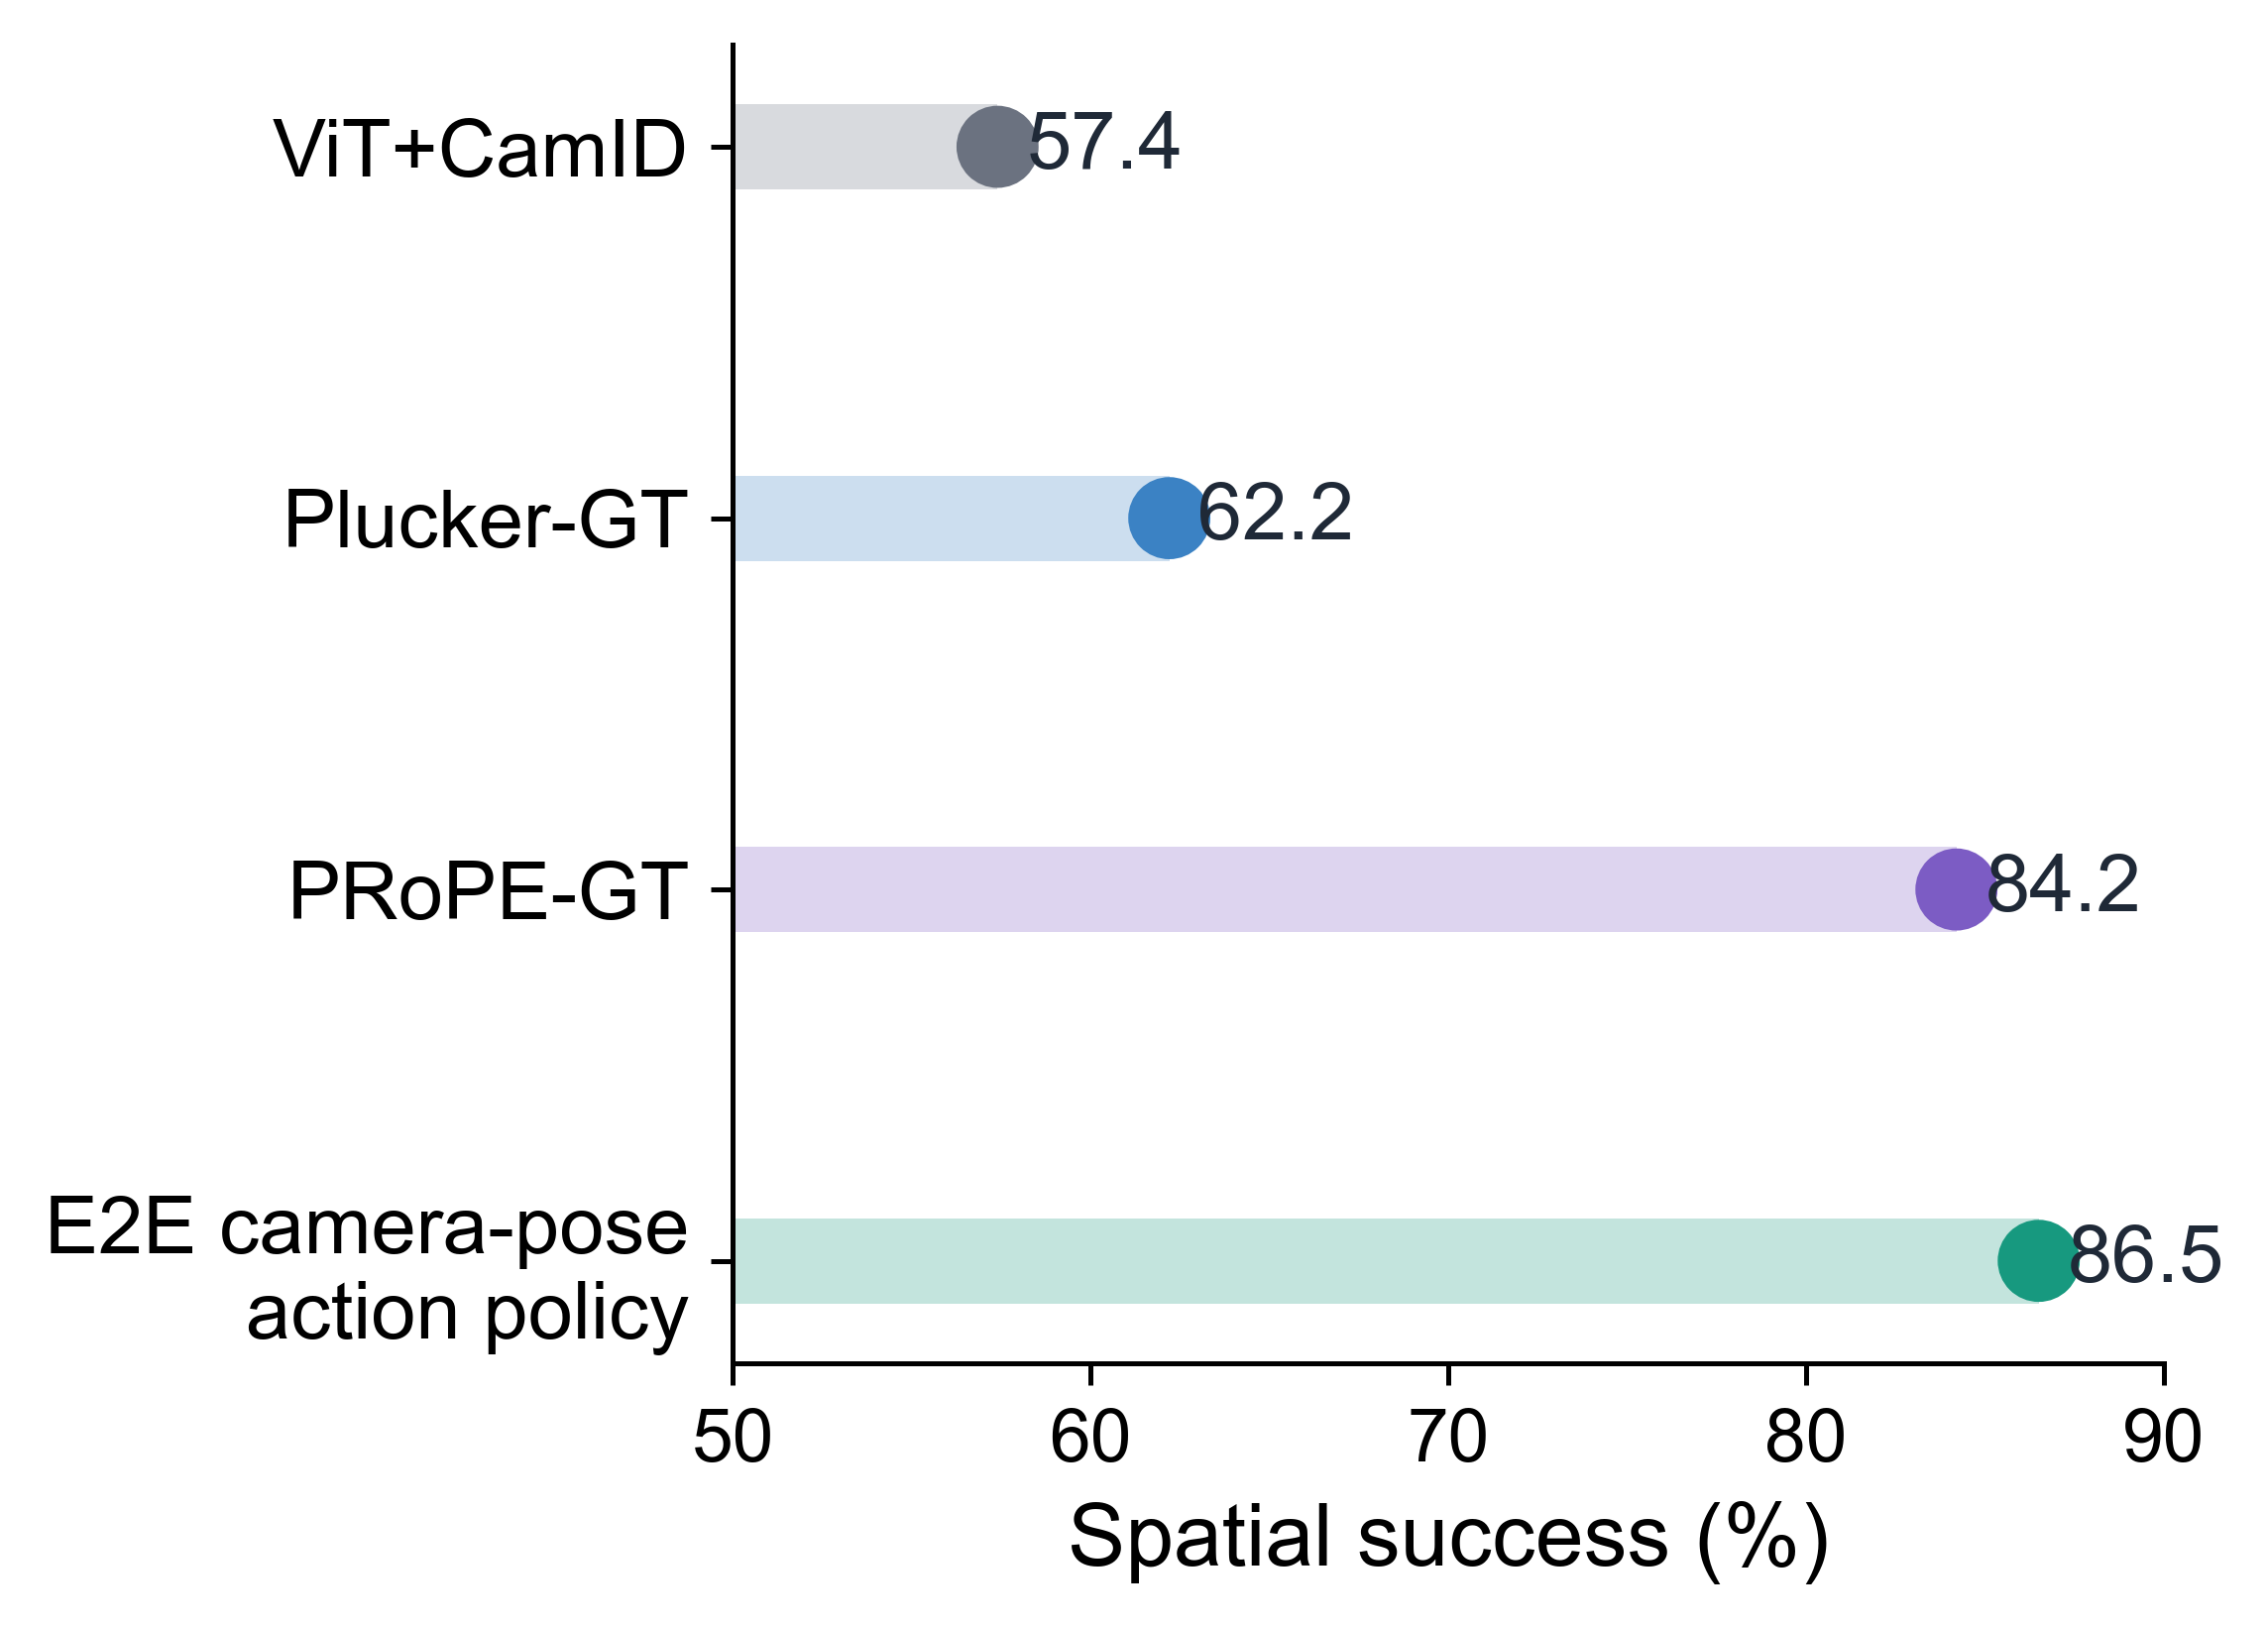
\includegraphics[width=0.95\linewidth]{figures/libero_mv_spatial_summary.png}
  \caption{LIBERO-MV Spatial summary. Left: calibrated references from the Camera-Aware Multi-View Visuomotor Policies protocol and the best current E2E camera-pose action policy. Right: episode-level success as the fraction of camera-pose-labeled training episodes varies.}
  \label{fig:libero}
\end{figure}

\subsection{MimicGen Camera-Shift Evaluation}

\paragraph{Dataset and splits.}
MimicGen is our main camera-shift benchmark because it lets us render the same
task family under controlled training and evaluation camera distributions.  We
currently report four tasks: Stack Three, Coffee, Threading, and Stack.  Each
policy is trained on the corresponding MimicGen multicamera demonstrations with
12 random surround cameras available per episode.  We use a deterministic
demo-level validation split with \(5\%\) held out by
\(\mathrm{md5}(\texttt{split\_seed},\texttt{dataset\_path},\texttt{demo\_key})\)
and split seed 0.  The training dataloader uses only the train split; rollout
evaluation can draw initial states from either split.  The results in
Fig.~\ref{fig:mimicgen-prelim} use train-split initial states so camera-shift,
rather than unseen object initialization, is the isolated variable.  We also log
validation-split initial-state rollouts with the same two camera modes, but do
not include them in the current main figure.

\paragraph{Camera distributions.}
Each training sample draws views from the \texttt{train\_wide} camera
distribution.  This distribution samples 12 look-at cameras with distance in
\([0.25,1.5]\) m, height offset in \([-0.3,1.0]\) m, \(45^\circ\) vertical field
of view, and up to 0.15 m target jitter; it does not reject views that only
partially cover the workspace.  The held-out \texttt{eval\_tight} distribution
uses a different, narrower camera band: distance in \([0.65,0.95]\) m, height
offset in \([0.15,0.45]\) m, 0.05 m target jitter, and a visibility filter that
requires a \(0.40{\times}0.40{\times}0.20\) m workspace box to project inside
the image with an 8-pixel margin.  Both distributions render \(128{\times}128\)
RGB images.  At rollout time we evaluate each checkpoint under both
\texttt{train\_wide} and \texttt{eval\_tight}, 40 rollouts per cell, with the
same seed base and 8-step action execution interval.

\paragraph{Methods and inputs.}
Diffusion Policy is the image-only baseline: it receives RGB observations and
proprioception but no explicit 3D or camera-pose input.  ManiFlow is the
point-cloud baseline and is the only method in Fig.~\ref{fig:mimicgen-prelim}
that consumes point clouds.  The E2E camera-pose action policy receives RGB,
predicts camera poses internally, converts them into Plucker ray maps, and
trains with action and semi-supervised pose losses.  In the current MimicGen
configuration it uses two surround cameras plus the wrist camera, 50\%
episode-level pose labels, teacher forcing during pose warmup, and predicted
poses afterward.  The E2E camera-pose NVS policy uses the same pose-label ratio
and adds the scene-token NVS branch.  Its current register-token configuration
keeps 64 active scene tokens, samples one target input view for reconstruction,
and drops the target observation from the encoder with probability 0.6 by
zeroing both RGB and Plucker channels.  The NVS decoder is used only during
training.

\paragraph{Results.}
Fig.~\ref{fig:mimicgen-prelim} reports the current multi-task result set.  Hammer
Cleanup is omitted because this round focuses on the four completed tasks.  The
final group reports a macro-average over the displayed tasks.  The NVS policy
improves over the E2E camera-pose action policy by 13.1 percentage points on
train-camera evaluation and 23.1 points under tight-camera evaluation.  On
Stack, it matches the action-only variant on train-camera evaluation at 97.5\%
success and improves tight-camera success from 2.5\% to 42.5\%.

\begin{figure}[t]
  \centering
  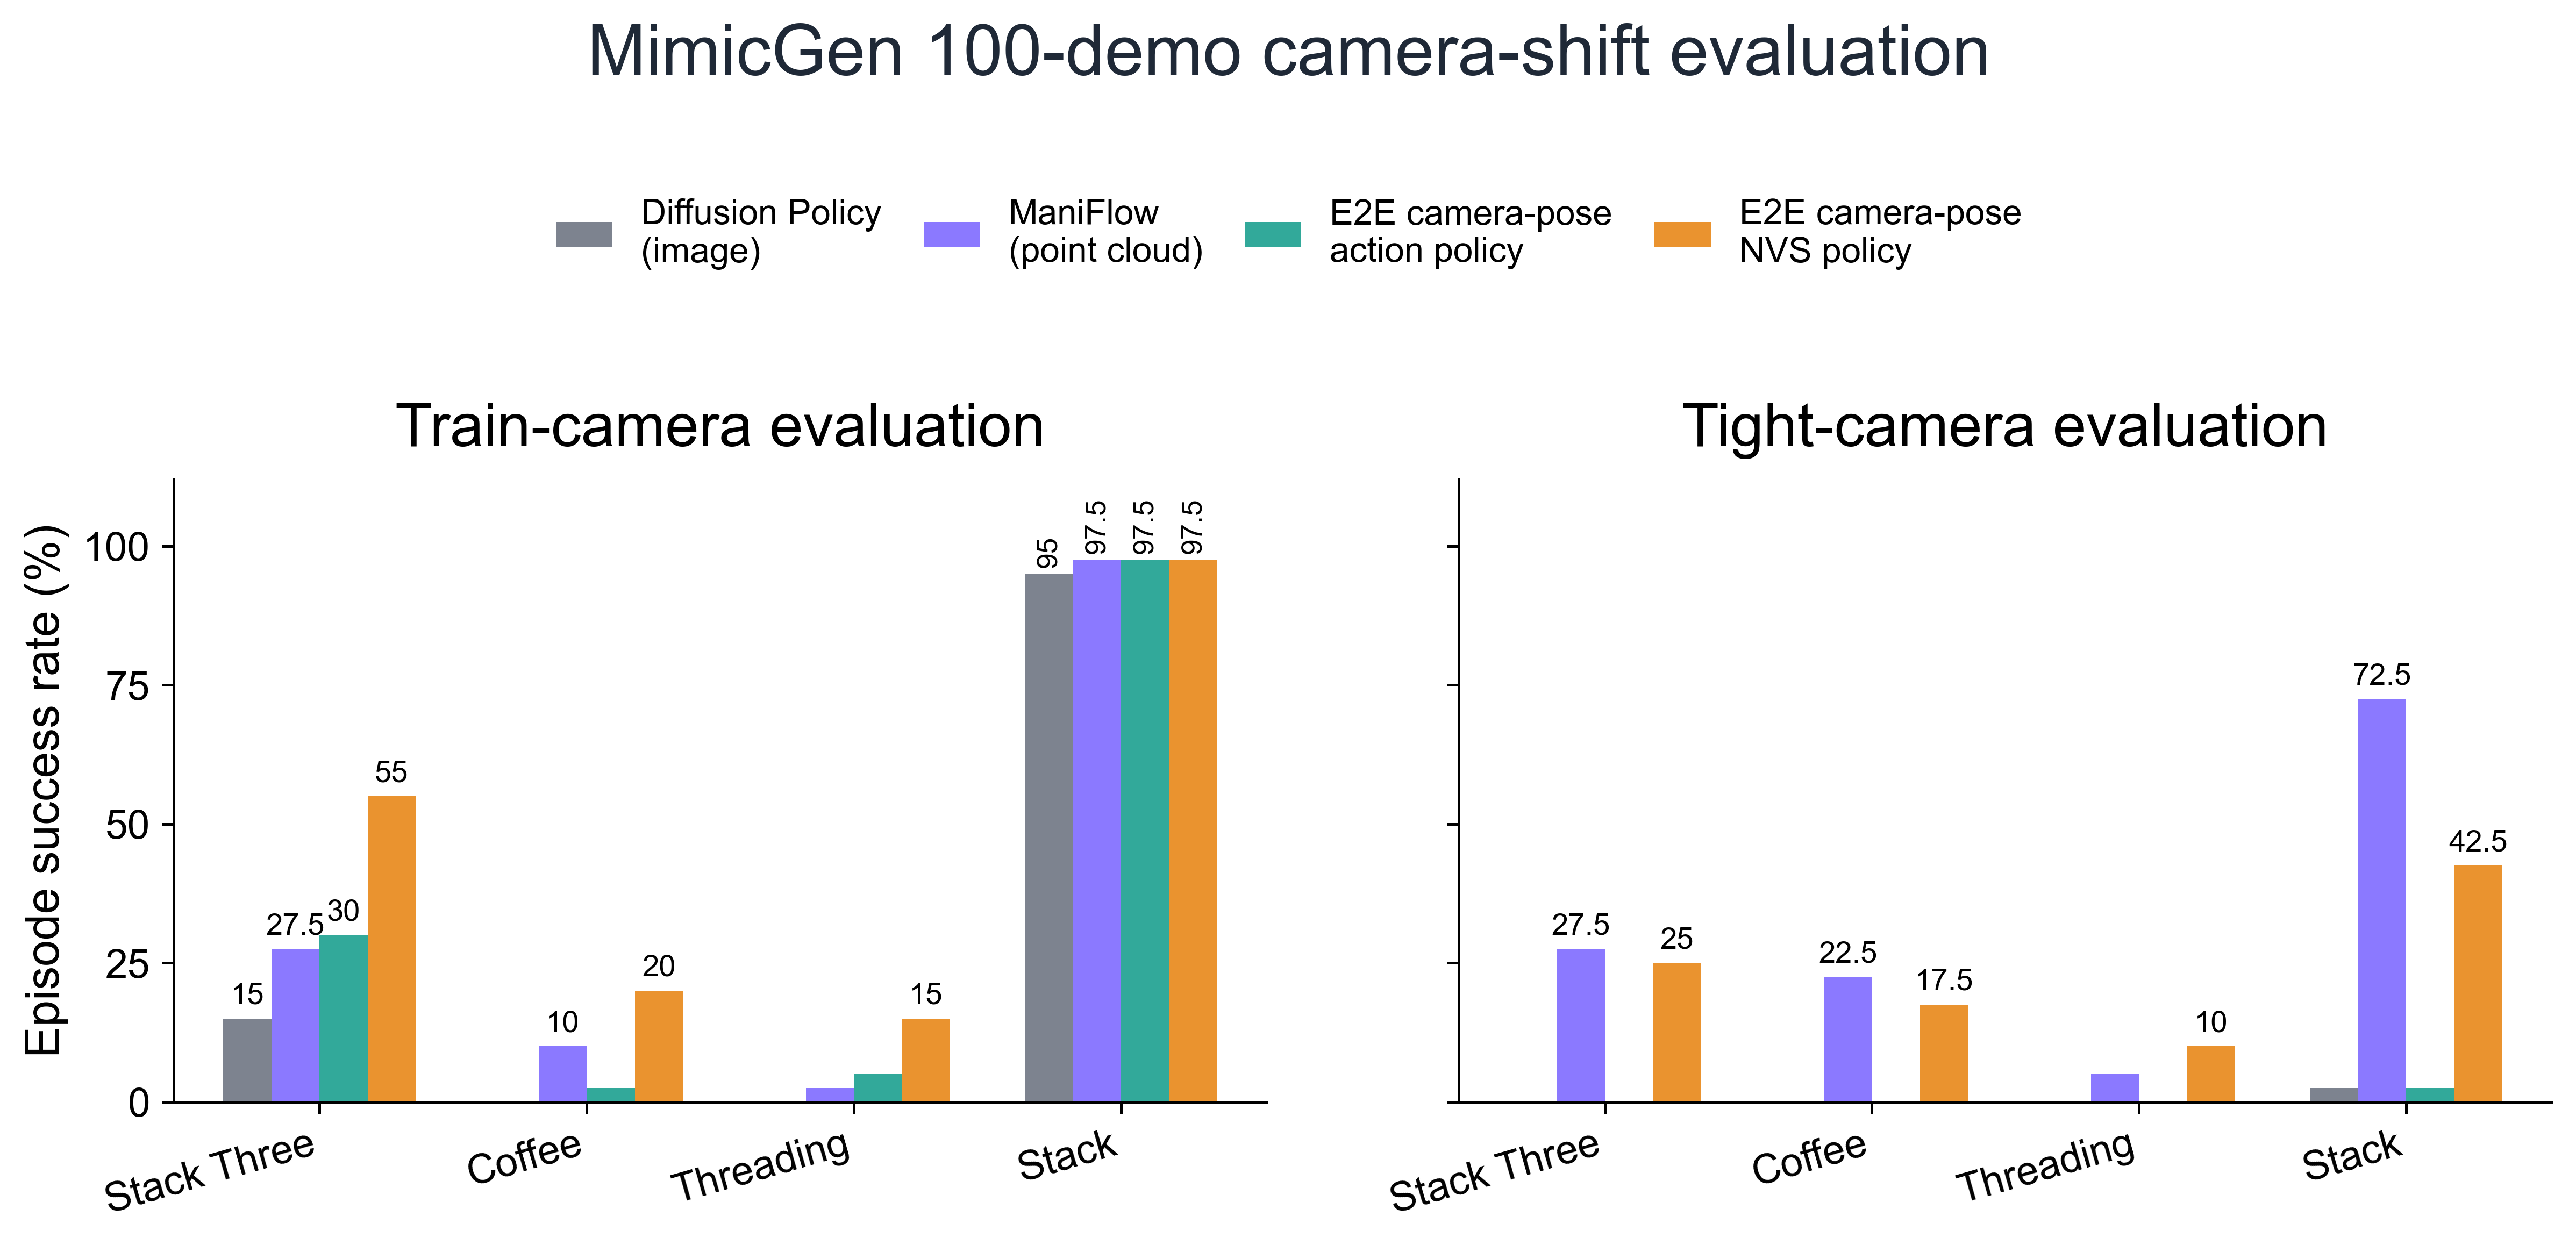
\includegraphics[width=\linewidth]{figures/mimicgen_multitask_results.png}
  \caption{Preliminary MimicGen results. Bars report episode-level success rates under the train-camera and tight-camera camera distributions; the shaded Mean group is the macro-average over the four displayed tasks. Diffusion Policy is an image baseline, ManiFlow is a point-cloud baseline, and the two E2E variants match the model names in Fig.~\ref{fig:pipeline}.}
  \label{fig:mimicgen-prelim}
\end{figure}

\subsection{Real-World Tabletop Evaluation}

\paragraph{Protocol.}
We also run an initial real-world tabletop evaluation following the hardware,
camera, and scoring setup of Camera-Aware Multi-View Visuomotor
Policies~\citep{anonymous2026cameraaware}.  The platform is a single-arm
Trossen WidowX AI in an ALOHA-style leader--follower setup.  The observation
stream contains one wrist Intel RealSense D405 camera and two scene-side Intel
RealSense D455F cameras.  The referenced setup trains from teleoperated
episodes resampled to a 50 Hz state/action clock, predicts 1-second action
chunks, and represents each action as position, 6D rotation, and continuous
gripper command.  For Blocks-in-Bowl, the trial has a 4-minute wall-clock cap.
The rubric gives one point per successful grasp and one point per successful
placement across four blocks, for eight progress points per trial; full-task
success requires all four blocks to be placed in the bowl.

\paragraph{Comparison.}
For the first comparison in Fig.~\ref{fig:realworld-blocks}, we use only the
reported calibrated Plucker-GT Blocks-in-Bowl result from the under-review
paper.  That baseline receives calibrated scene-camera extrinsics and reports
50\% full-task success and 86\% rubric-weighted task progress over 10 trials.
Our current E2E camera-pose NVS policy is evaluated under the same success
definition and trial count, but predicts camera geometry inside the policy
rather than using calibrated Plucker maps as fixed input.  The current run
reaches 100\% full-task success on Blocks-in-Bowl.  Because this is one task
and one 10-trial run, we treat it as an initial hardware check rather than a
complete real-world benchmark.

\begin{figure}[t]
  \centering
  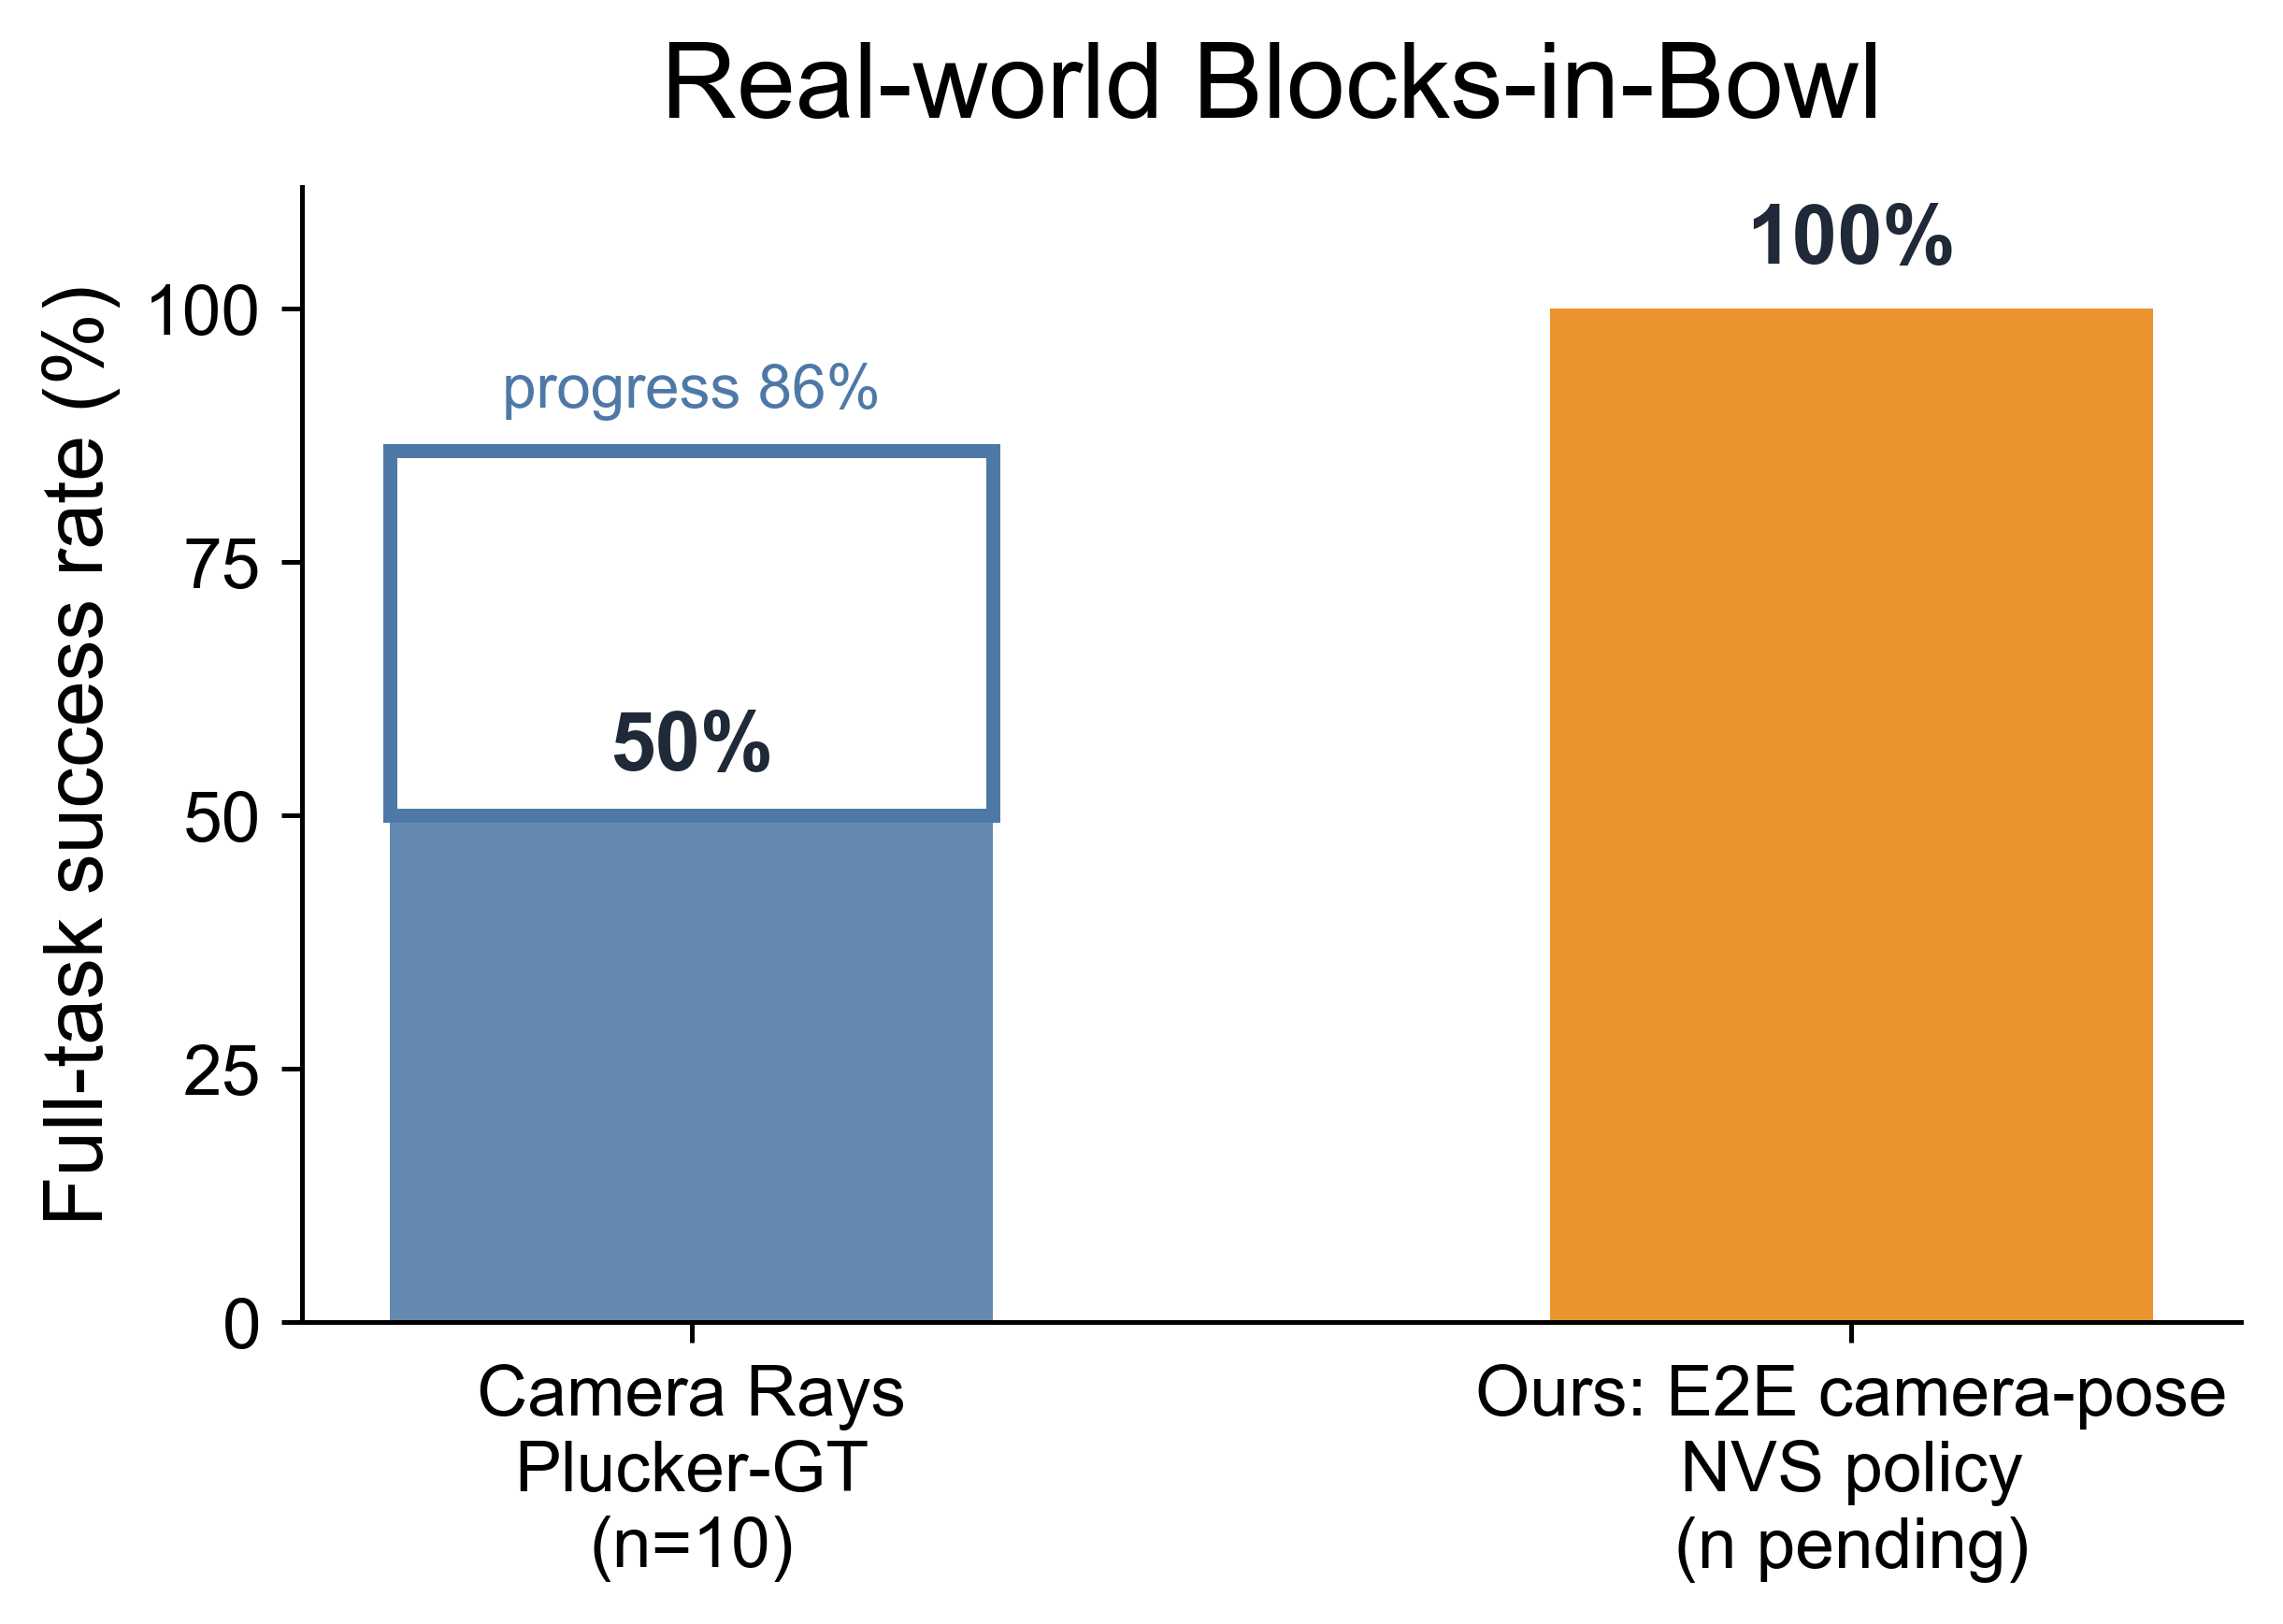
\includegraphics[width=0.68\linewidth]{figures/realworld_blocks_bowl_comparison.png}
  \caption{Initial real-world Blocks-in-Bowl comparison under the same 10-trial success definition. The Camera Rays number is the reported calibrated Plucker-GT result; the outlined extension shows their task-progress score.}
  \label{fig:realworld-blocks}
\end{figure}
